\subsection{Introduction}
Over the last decade cloud computing has become a popular approach for deploying
applications at scale. Many organizations, academic institutions, and hobbyists make use of public
and/or private clouds to deploy their applications.
This rapid growth in cloud technology has intensified the need 
for new techniques to
monitor applications deployed in cloud platforms. Application developers and users wish
to monitor the availability of the deployed applications, track application performance, and detect 
application and system anomalies as they occur. To obtain this level of deep operational insight into
cloud-hosted applications, the cloud platforms must be equipped with powerful instrumentation,
data gathering and analysis capabilities that span the entire stack of the cloud. 
Moreover, clouds must provide comprehensive
data visualization and notification mechanisms. However, most cloud technologies available
today either do not provide any application monitoring support, or only provide primitive
monitoring features such as application-level logging. Hence, they are not capable of performing
powerful predictive analyses or anomaly detection, which require much more fine-grained, low-level
and systemwide data collection and analytics. 

Further compounding this problem, today's cloud platforms are very large and complex. They are
comprised of many layers, where each layer may consist of a multitude of interacting components.
Therefore when a performance anomaly manifests in a user application, it is rather challenging 
to determine the exact layer or the component of the cloud platform that may be responsible for it. 
Facilitating this level of comprehensive root cause analysis requires
data collection at different layers of the cloud, and mechanisms for correlating events at
different layers and components. Today's cloud platforms do not support such deeply integrated
data collection. The plethora of existing third party cloud monitoring solutions
do not have access to low-level data regarding the cloud thereby rendering them incapable
of performing systemwide root cause analysis.

Moreover, performance monitoring for cloud applications needs to be highly customizable. Different
applications have different monitoring requirements in terms of data gathering frequency, 
length of the history to consider when performing statistical analysis, and the performance 
SLAs to maintain over time and check for violations. It should also be possible to easily extend
cloud application monitoring frameworks with
new statistical analysis methods and algorithms for detecting application performance
anomalies, and performing root cause analysis. Designing such customizable and extensible performance
monitoring frameworks that are built into the cloud platforms is a novel yet challenging undertaking.

To address these needs, we present the design of 
a comprehensive application platform 
monitor (APM) called Roots that can be easily integrated with a wide variety of cloud Platform-as-a-Service 
(PaaS) technologies. The proposed
APM is not an external system that monitors a cloud platform from the outside (as most APM systems today). 
Rather, it integrates with
the PaaS cloud from within thereby extending and augmenting the existing components of the PaaS cloud
to provide comprehensive full stack monitoring and analytics. 
We believe that this design decision is a key differentiator over existing cloud 
application monitoring systems because (i) it is
able to take advantage of the scaling, efficiency, deployment, fault tolerance, security, 
and control features that the underlying cloud offers, 
(ii) while providing low overhead end-to-end monitoring and analysis of cloud applications.

PaaS clouds execute web-accessible (HTTP/S) applications, to which they provide 
high levels of scalability, availability, and execution management. 
PaaS clouds provide scalability by automatically allocating resources 
for applications on the fly (auto scaling), and provide availability through
the execution of multiple instances of the application and/or the PaaS
services they employ for their functionality.
Consequently, viable PaaS technologies as well as
PaaS-enabled applications continue to increase rapidly in number~\cite{paas-growth}.
PaaS clouds provide a high level of abstraction to the application developer that effectively hides
all the infra\-structure-level details such as physical resource allocation (CPU, memory, disk etc), operating
system,
and network configuration. This enables application developers to focus solely on the programming
aspects of their applications, without having to be concerned about deployment issues. But
due to this high level of abstraction, performance monitoring and root cause analysis
is particularly challenging in PaaS clouds. Due to this reason, and the large number of 
PaaS applications available for testing, we design Roots APM to operate within PaaS
clouds.

Roots is highly customizable so that different monitoring policies can be
configured at the application level. It also facilitates a number of statistical analysis
methods for anomaly detection and root cause analysis. New analysis methods
can be easily brought into the framework by building on the high-level abstractions
that Roots provides. This enables us to experiment with different combinations of
statistical methods to determine which analysis works best for a given application or
SLA scenario. Roots collects most of the data it requires by instrumenting 
various components of the cloud platform. However, it takes special care to keep the data
collection overhead to a minimum. To this end it does not instrument any user code (i.e. applications)
deployed in the cloud. On a related note, it also does not impose any restrictions on the user code.
That is, the developer does not have to write code using some Roots-specific API or link their
code with a Roots-specific library. Any application that can run on the cloud platform without Roots, can
be monitored and analyzed by Roots with no code changes necessary. 

Roots uses batch operations and asynchonous 
communication whenever possible to record events in a manner that does not introduce
delays to the application request processing activities carried out by the 
PaaS cloud. 
Additionally, Roots employs a collection of lightweight continuous application benchmarking
processes to collect performance data regarding user applications. Both
the benchmarking processes, and the data analysis processes are executed 
out of the request processing flow of the cloud platform. Such processes can be
grouped together, and managed by a single deployable entity known as a
``Roots Pod''. Pods are specifically designed to keep minimum state
information regarding the applications they monitor and analyze. This enables
a single pod to monitor a large number of applications. Each pod is self-contained,
and therefore scalability and high availability can be achieved by running multiple pods (sharding),
and running multiple replicas of the same pod.

The following subsections detail the architecture of Roots APM, and how it integrates with a typical PaaS
cloud. We describe individual components of the APM, their functions and how they interact with each
other. Where appropriate, we also detail the concrete technologies (tools and products) that we plan to use to implement
various components of the APM, and provide our rationale and intuition behind choosing these technologies.

\subsection{PaaS System Organization}
\begin{figure}
\centering
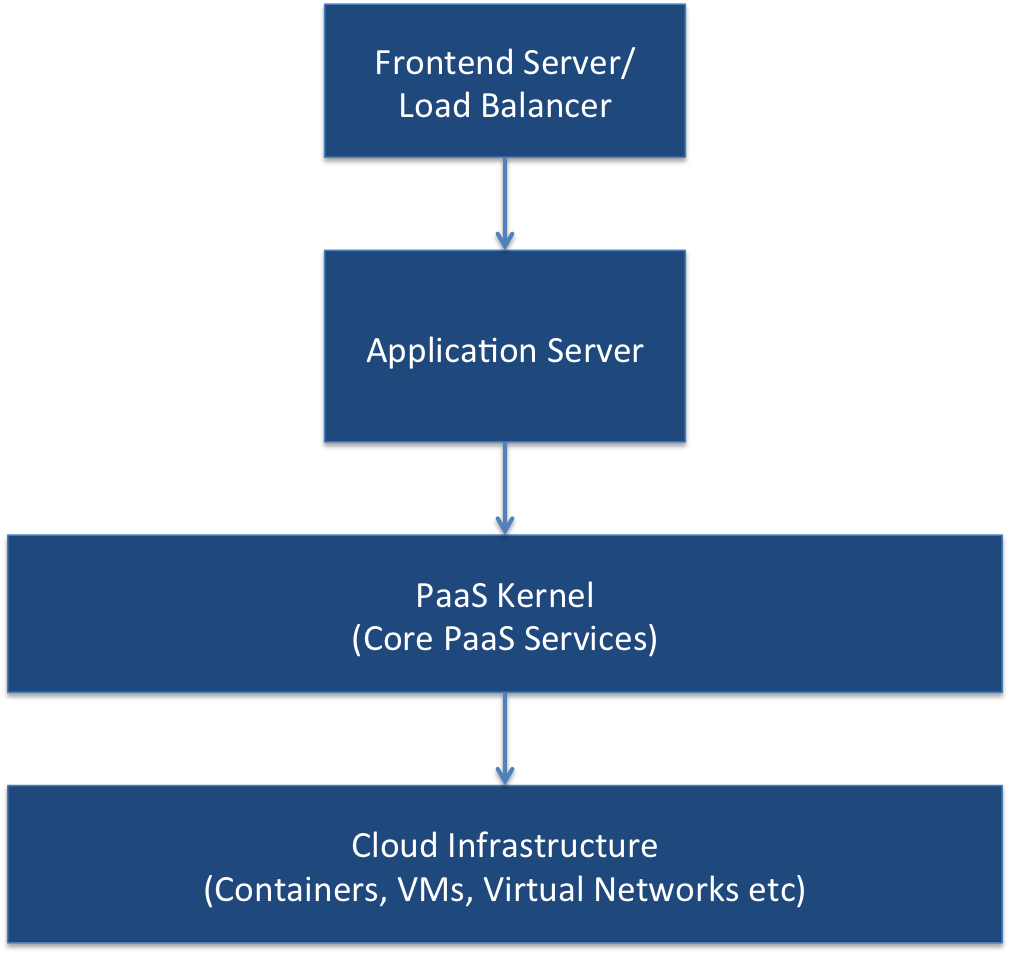
\includegraphics[scale=0.5]{paas_architecture}
\caption{PaaS system organization.}
\label{fig:paas_architecture}
\end{figure}

Figure~\ref{fig:paas_architecture} shows the key layers of a typical PaaS cloud. Arrows indicate
the flow of data and control in response to application requests.

At the lowest level of a PaaS cloud is an infrastructure that consists of the necessary compute, storage
and networking resources. How this infrastructure is set up may vary from a simple cluster of physical 
machines to a comprehensive Infrastructure-as-a-Service (IaaS) solution. In large scale PaaS clouds,
this layer typically consists of many virtual machines and/or containers with the ability to acquire more
resources on the fly.

On top of the infrastructure layer lies the PaaS kernel. This is a collection of managed, scalable
services that high-level application developers can compose into their applications. The provided services
may include database services, caching services, queuing services and much more. Some PaaS clouds
provide a managed set of APIs (an SDK) for the application developer to access these fundamental services. 
In that case all interactions between the applications and the PaaS kernel must take place through
the cloud provider specified APIs (e.g. Google App Engine). 

One level above the PaaS kernel we find the application servers that are used to deploy and run
applications. Application servers provide the necessary integration (linkage) between application code and the
underlying PaaS kernel, while sandboxing application code for secure, multi-tenant operation. On top
of the application servers layer resides the fronted and load balancing layer. This layer is responsible
for receiving all application requests, filtering them and routing them to an appropriate application
server instance for further execution. As the fronted server, it is the entry point for PaaS-deployed
applications for all application clients.

Each of the above layers can span multiple processes, running over multiple physical or virtual
machines. Therefore the execution of a single application request typically involves cooperation
of multiple distributed processes and/or machines. In order to perform comprehensive monitoring
and root cause analysis, we need to be able to monitor each of the above layers along with their
enclosed components. Further we need to be able to trace the flow of data and control
across different layers and components.

\subsection{Roots Cloud APM Architecture}
\subsubsection{Key Functions and Requirements}
\begin{figure}
\centering
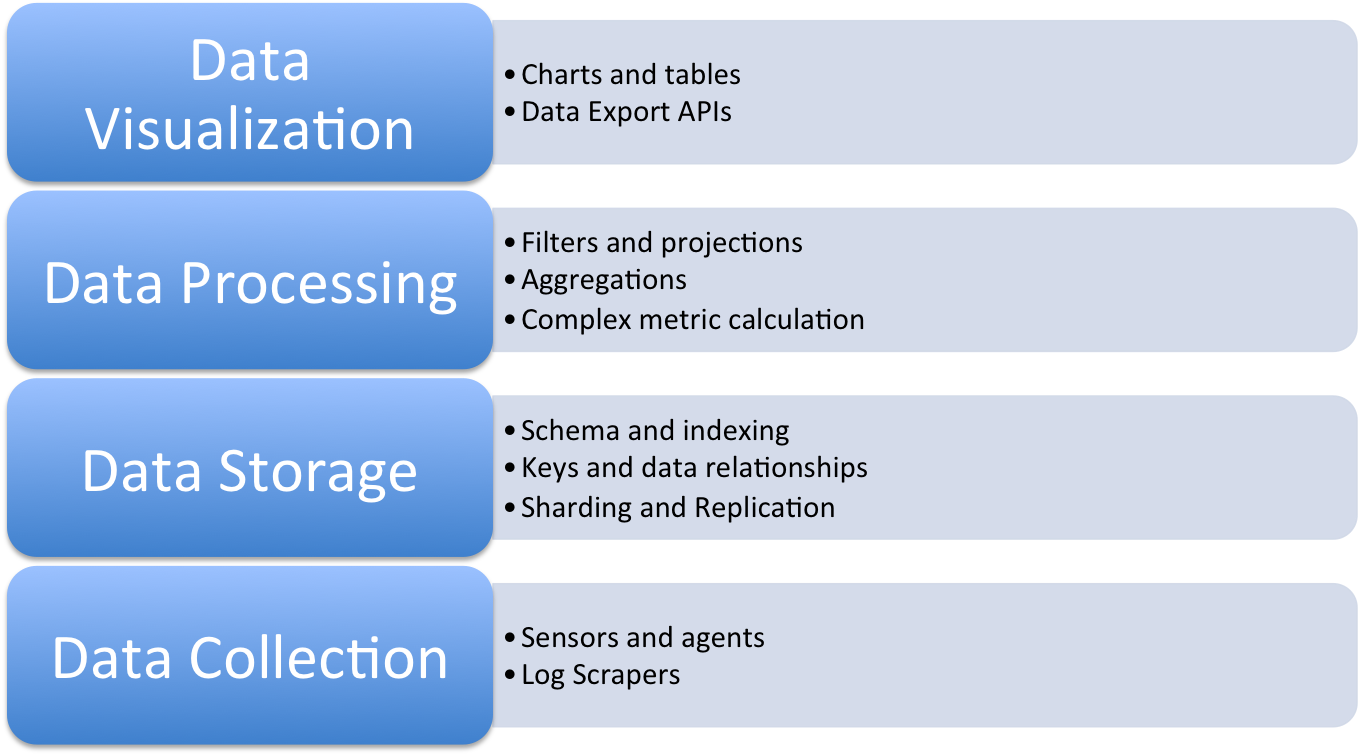
\includegraphics[scale=0.5]{apm_functions}
\caption{Key functions of the Roots APM.}
\label{fig:apm_functions}
\end{figure}

\begin{figure}
\centering
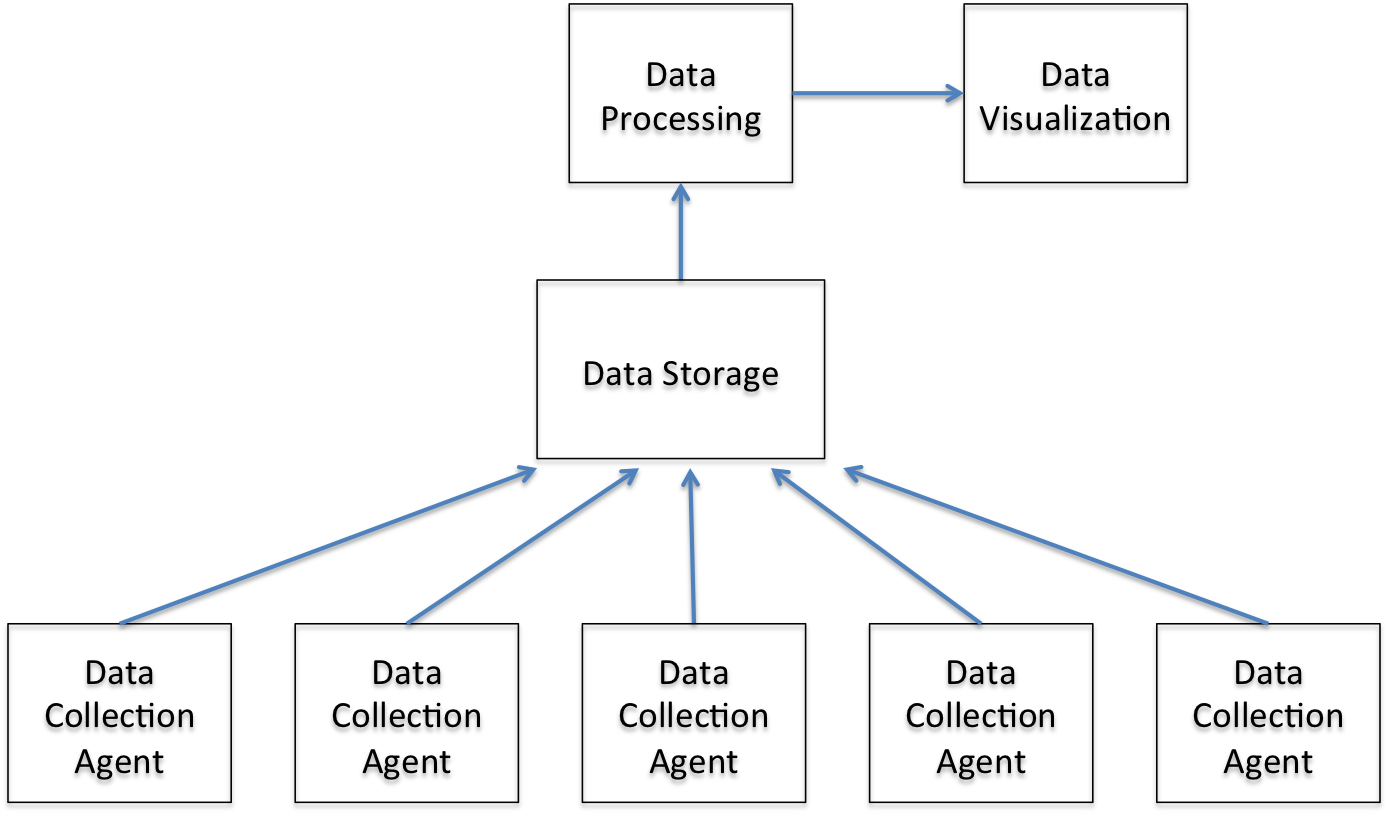
\includegraphics[scale=0.5]{apm_layout}
\caption{Deployment view of the Roots APM functions.}
\label{fig:apm_layout}
\end{figure}

Like most system monitoring solutions, the proposed cloud APM must serve four major functions: Data
collection, storage, processing (analytics) and visualization. Figure~\ref{fig:apm_functions} shows the
logical organization of these functions in the APM, and various tasks that fall under each of them.
Figure~\ref{fig:apm_layout} shows a physical deployment view of the said functions. Arrows indicate
the flow of information through the APM.

Data collection is performed by various sensors and agents that instrument the
core components of the PaaS cloud.
While sensors are very primitive in their capability to monitor
a given component, an agent may intelligently adapt to changing conditions, making decisions on
what information to capture and how often. 
Monitoring and instrumentation should be lightweight and as non-intrusive
as possible so their existence does not impose additional overhead 
on the applications. Specifically, we avoid instrumenting application code in Roots to prevent
introducing an additional overhead to the application execution. 

Data storage components should be capable of
dealing with potentially very high volumes of data. The data must be organized and indexed
to facilitate efficient retrieval, and replicated to maintain reliability and high availability. 
Additionally, Roots should also support timely removal of old data (i.e. garbage collection)
in an efficient and non-invasive manner.

Data processing components should also be capable of processing large volumes of data in near real-time,
while supporting a wide range of data analytics features such as filters, projections and aggregations. 
They will employ various statistical and perhaps even machine learning methods to understand the
data, detect anomalies and identify bottlenecks in the system. Roots should also provide high-level
abstractions so that new data analysis methods can be implemented when necessary.

Data visualization layer mainly consists of graphical interfaces (dashboards) for displaying various
metrics computed by the data processing components. Additionally it may also have APIs to export
the calculated results and trigger alerts. 

\subsubsection{APM Architecture and Integration with PaaS Clouds}
\begin{figure}
\centering
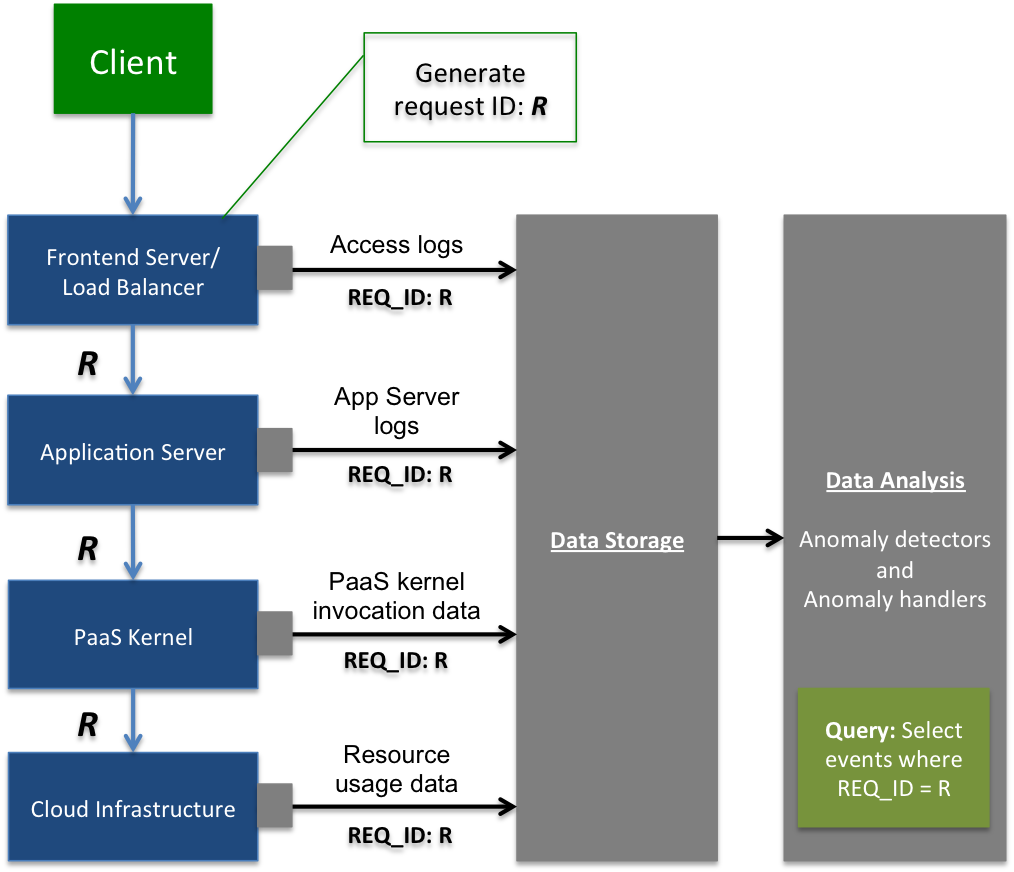
\includegraphics[scale=0.35]{apm_architecture}
\caption{APM architecture.}
\label{fig:apm_architecture}
\end{figure}

Figure~\ref{fig:apm_architecture} illustrates the overall architecture of the proposed APM, and how 
it fits into the PaaS cloud stack. APM components are shown in grey, with their interactions indicated
by the black lines. The small grey boxes attached to the PaaS components represent the sensors and
agents used to instrument the cloud platform for data collection purposes. Note that the APM collects
data from all layers in the PaaS stack (i.e. full stack monitoring).

From the front-end and load balancing layer we gather all information related to incoming application
requests. A big part of this is scraping the HTTP server access logs, which indicate request timestamps,
source and destination addressing information, response time (latency) and other HTTP message
parameters. This information is readily available for harvesting in most technologies used as front-end
servers (e.g. Apache HTTPD, Nginx). Additionally we may also collect information pertaining to active
connections, invalid access attempts and other errors.

From the application server layer we intend to collect basic application logs as well as any other logs and 
metrics that can be easily collected from the application runtime. This may include some process level
metrics indicating the resource usage of the individual application instances. Additionally Roots
employs a collection per-application benchmarking processes, that periodically probes applications
to measure their performance. These are lightweight, stateless processes managed by the Roots framework.
Data collected by these processes will also be sent to data storage component, and will be available
for analysis as per-application timeseries data.

At the PaaS kernel layer we employ instrumentation to record information regarding all kernel invocations
made by the applications. This instrumentation must be applied carefully as to not introduce a noticeable
overhead to the application execution. For each PaaS kernel invocation, we can capture the 
following parameters.
\begin{itemize}
\item Source application making the kernel invocation
\item Timestamp
\item Target kernel service and operation
\item Execution time of the invocation
\item Request size, hash and other parameters
\end{itemize}
Collecting this PaaS kernel invocation details enables tracing the execution of application 
requests, without the need for instrumenting application code, which we believe is a feature 
unique to PaaS clouds. 

Finally, at the lowest infrastructure level, we can collect information related to virtual machines, containers
and their resource usage. We can also gather metrics on network usage by individual components which
might be useful in a number of traffic engineering use cases. Where appropriate we can also scrape
hypervisor and container manager logs to get an idea of how resources are allocated and released over
time. However, we will not investigate data collected at this level in our immediate future work.
To begin with we wish to perform anomaly detection at the frontend and application server levels, and conduct
root cause analysis at the PaaS kernel level.

To summarize, the types of services and resources that Roots will be able
to monitor include the following. Moreover, our design of the Roots data collection 
layer is abstract and thus easily extended to permit monitoring of new services 
and PaaS components as they become available in the future.
\begin{itemize}
\item Cloud Infrastructure: 
  \begin{itemize}
  \item CPU, memory, disk, network
  \item Linux containers, virtual machines
  \end{itemize}
\item PaaS Kernel (including PaaS cloud SDK)
  \begin{itemize}
  \item Task queues, security components (user/developer tracking and authentication and authorization)
  \item Data caches, datastores (key value, NoSQL), databases (fixed schema, SQL).
  \end{itemize}
\item Application servers
  \begin{itemize}
  \item language-specific runtime systems
  \end{itemize}
\item Front-end components
  \begin{itemize}
  \item HTTP/S request serving 
  \item Load balancing and rate limiting components
  \end{itemize}
\end{itemize}

To avoid introducing delays to the application request processing flow, we implement
all Roots agents and sensors as asynchronous tasks. That is, none of them would
suspend application request processing to report data to the data storage components.
We make sure that all expensive I/O tasks related to data collection and storage is
executed out of the request processing flow.
In particular, all data is collected into log files or memory buffers that are local to the components being
monitored. This locally collected (or buffered) data will be periodically sent
to the data storage components of Roots using separate background tasks and batch communication
operations. Also special care is taken to isolate the activities in the cloud from potential
faults and failures in the Roots data collection or storage layers. 

\subsubsection{Cross-layer Data Correlation}
Previous subsection details how the APM collects useful monitoring data at each layer of the cloud
stack. To make most out of the gathered data, and use them to perform complex analyses, 
we must be able to correlate data records collected at different layers of the PaaS. For example consider
the execution of a single application request. This single event results in following data records at
different layers of the cloud, which will be collected and stored by the APM as separate entities.

\begin{itemize}
\item A front-end server access log entry
\item Zero or more application log entries
\item Zero or more PaaS kernel invocation records
\end{itemize}

We require a mechanism to tie these disparate records together, so the data processing layer can easily
aggregate the related information. For instance, we must be able to retrieve via an
aggregation query, all PaaS kernel invocations made by a specific application request.

To facilitate this requirement we propose that front-end server tags all incoming application requests 
with unique identifiers.
This request identifier can be attached to HTTP requests as a header which is visible to all components 
internal to the PaaS cloud. All data collecting agents can then be configured to record the request identifiers
whenever recording an event. At the data processing layer APM can aggregate the data by request identifiers
to efficiently group the related records.

\subsubsection{Data Analysis}
Roots data analysis layer uses two basic abstractions:
\begin{itemize}
\item Anomaly detector
\item Anomaly handler
\end{itemize}

Anomaly detectors are processes that periodically analyze the data collected for
each deployed application. Roots supports multiple detector implementations, where each implementation
uses a different statistical method to look for performance anomalies. Detectors are configured
at application level making is possible for different applications to use different anomaly 
detectors. Roots also supports multiple concurrent anomaly detectors on the same application, which can be used
to evaluate the efficiency of different detection strategies for any given application. Each
anomaly detector has an execution schedule (e.g. run every 60 seonds), and a sliding window 
(e.g. from 10 minutes ago to now)
associated with it. The boundaries and the length of the window determines the time range
of the data processed by the detector at any round of execution. Window is updated 
after each round of execution.

In addition to the various statistical anomaly detectors, Roots provides a special
``path anomaly detector'', that can be configured on any application. This detector
analyzes the sequences of PaaS SDK calls made by an application, and identifies the
different paths of execution that has resulted due to application request processing.
Each SDK call sequence corresponds to a path of execution through the application code.
This detector computes the frequency distribution of different paths (i.e. how often each path
gets executed), and checks how the distribution changes over time. By doing so the path anomaly
detector can identify the occurance of new paths (a type of novelty detection), most
frequently executed paths and
significant changes in the path frequency distribution. Such changes are usually
the results of changes in the nature of the application workload (e.g. from a readonly
workload to a readwrite workload in a data management application). 
This level of deep insight into application
performance and workload is possible in Roots only due to its systemwide data
collection and aggregation capabilities.

When an anomaly detector finds an anomaly in application performance, it sends an event
to a collection of anomaly handlers. The event encapsulates a unique anomaly identifier, 
timestamp, application identifier and the source detector's sliding window that correspond to the
anomaly. Anomaly handlers are configured globally (i.e. each handler
receives events from all detectors), but they can decide to not handle certain types
of anomaly events. Similar with detectors, Roots supports multiple anomaly handler
implementations -- one for logging anomalies, one for sending alert emails, one
for updating a dashboard etc. Additionally, Roots provides two special anomaly handler
implementations.
\begin{itemize}
\item Workload change analyzer
\item Root cause analyzer
\end{itemize}

The workload change analyzer analyzes the historical workload trends of the applications to
check if a particular anomaly is correlated with a recent change in the workload.
This is done by running a suite of changepoint detection algorithms on the workload
data captured by the Roots data collection layer. The root cause analyzer evaluates
the historical trend of PaaS SDK calls made by the application, and attempts to
determine the most likely components of the cloud (in the PaaS kernel) that may have 
attributed to a detected anomaly.

Both the anomaly detectors and anomaly handlers work with fix-sized sliding windows.
They are free to discard any old data as the sliding window moves along the time line.
As such the amount of state information these entities must keep in memory has
a strict upperbound. By doing so we make these processes lightweight. The old 
historical data can be kept persistently in the Roots data storage layer, until
they are deemed eligible for garbage collection.

The extensibility of Roots is primarily achieved through the abstractions of anomaly
detectors and handlers. Roots makes it simple to implement new detectors and handlers,
and plug them into the system. Both the detectors and the handlers are executed
as lightweight processes that do not interfere with the rest of the processes in
the cloud platform. Therefore failures in detectors and handlers have no impact
on the cloud platform or the deployed applications.

\subsubsection{Roots Process Management}
Most data collection activities in Roots can be treated as passive -- i.e. they
happen automatically as the applications receive and process requests in the cloud
platform. They do not require explicit scheduling or management. In contrast,
application benchmarking and data analysis are active processes that require
explicit scheduling and management.  This is achieved by grouping benchmarking
and data analysis processes into units called Roots pods. 

Each Roots pod is responsible for starting and maintainig a preconfigured set of
benchmarkers and data analysis processes (i.e. anomaly detectors and handlers). 
Each of these processes are light enough, so as to pack a large number of them
into a single pod. Pods are self-contained entities, and there is no inter-communication
between pods. Processes in a pod can efficiently communicate with each other 
(using shared memory), and call out to the Roots data storage to retrieve 
collected performance data for analysis. This enables starting and stopping 
Roots pods with minimal impact on the overall monitoring system. Furthermore, pods
can be replicated for high availability, and application load can be distributed
among multiple pods for scalability. For example, in a cloud platform with
1 million deployed applications, 100 pods can be used with each pod responsible
for running benchmarkers and analyzers for 10,000 applications.

To automate the process of managing pods, they can be tied into the core
process management framework of the PaaS cloud. That way whenever the cloud
platform initializes, a collection of pods can be started automatically.
Application deployment process of the PaaS cloud can be easily augmented
to register each new application with one of the available pods, so that the
benchmarkers and anomaly detectors can start running on the application.
Moreover, pods can be moved around or restarted as needed in response
to errors and autoscaling events that occur in the cloud platform.

\subsection{Implementation}
\begin{figure}
\centering
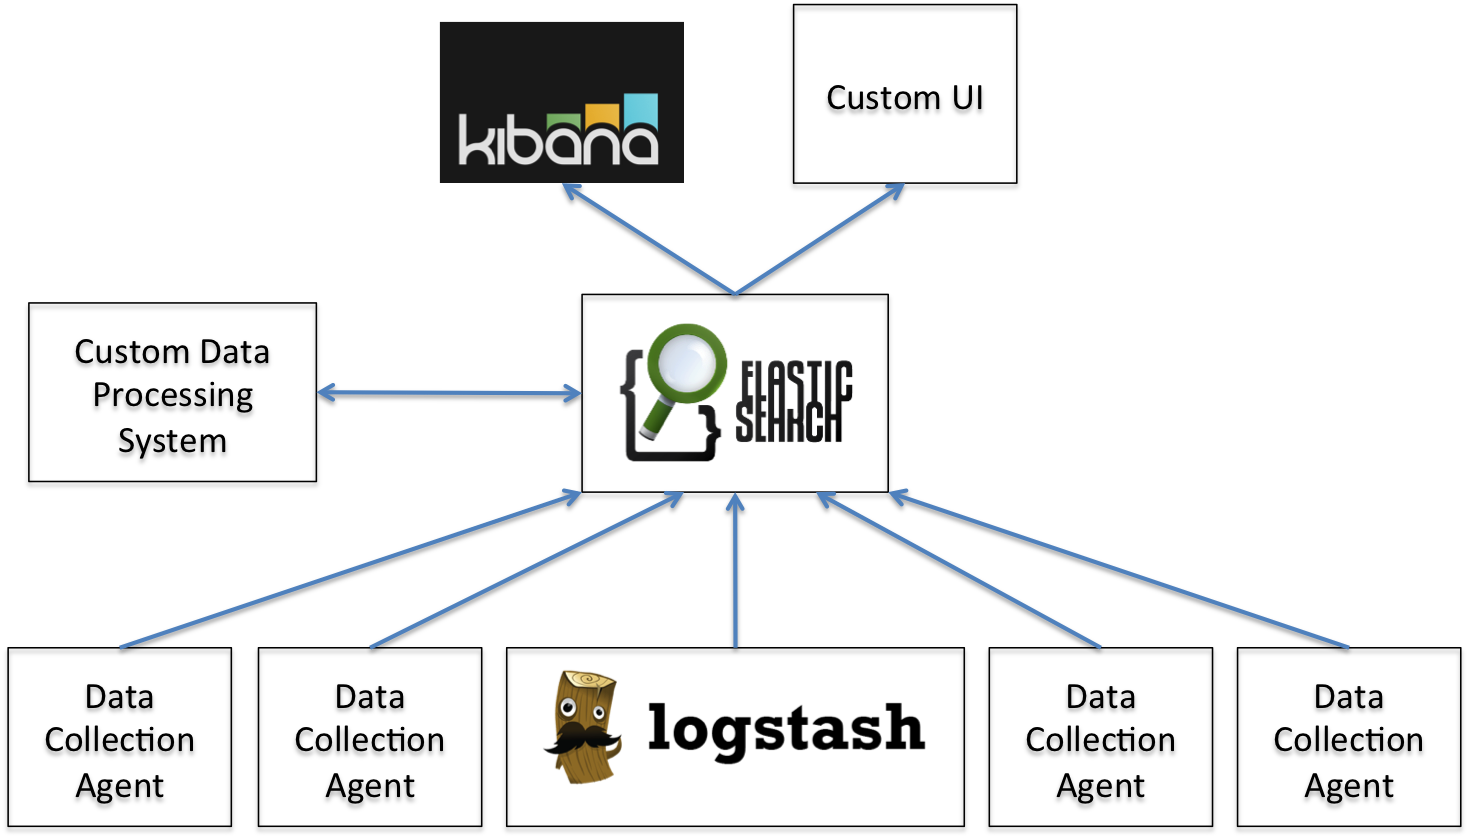
\includegraphics[scale=0.5]{apm_impl}
\caption{APM implementation based on ElasticSearch.}
\label{fig:apm_impl}
\end{figure}

\subsubsection{Data Collection, Storage and Visualization}
In this section we outline some of the technologies and tools that we have chosen to implement the proposed
APM architecture.  After a thorough evaluation of numerous existing system monitoring tools and platforms, 
we have decided to implement our APM for PaaS clouds using ElasticSearch. More specifically, ElasticSearch
will operate as the primary data storage component of the APM. ElasticSearch is ideal for storing large volumes
of structured and semi-structured data. It supports scalability and high availability via sharding and replication.
Perhaps what makes ElasticSearch an excellent choice for an APM is its comprehensive data indexing and
query support. Using the tried and tested Apache Lucene technology, ElasticSearch continuously organizes
and indexes data, making the information available for fast retrieval and efficient querying. 
Additionally it also provides
powerful data filtering and aggregation features, which can greatly simplify the implementations of high-level
data processing algorithms.

Data can be directly stored in ElasticSearch via its REST API. This means most data collection agents can 
simply make HTTP calls to ElasticSearch to add new records. ElasticSearch also supports batch 
processing thereby enabling agents to locally buffer collected data, and store them in batches to avoid
making too many HTTP calls. For scraping server logs and storing the extracted records in ElasticSearch,
we can use the Logstash tool. Logstash supports scraping a wide range of standard log formats (e.g. 
Apache HTTPD access logs), and other custom log formats can be supported via a simple configuration.
It also integrates naturally with ElasticSearch.

For data visualization we are currently considering Kibana, a powerful web-based dash boarding tool 
that is specifically designed to operate in conjunction with ElasticSearch. Kibana provides a wide
range of charting and tabulation capabilities, with particularly strong support for temporal data.  Since
ElasticSearch exposes all stored data via its REST API, it's also possible to bring other visualization
tools into the mix easily.

Figure~\ref{fig:apm_impl} shows the APM deployment view with ElasticSearch and other related technologies
in place. Most of the data processing features are provided by ElasticSearch itself, and other more complex
data analytics can be provided by a custom data processing system.

\subsubsection{Data Analysis}
Roots pods are implemented as standalone Java server processes. Threads are used to run benchmarkers,
anomaly detectors and handlers concurrently within each pod. Pods communicate with ElasticSearch via
REST calls, and most of the data analysis tasks such as filtering and aggregation are performed
at ElasticSearch itself. By doing so most of the heavy computations can be offloaded to the 
ElasticSearch cluster, which is specifically designed for high-performance query processing
and analytics. The pod implementation remains simple, and their runtime overhead is kept
to a minimum.

\subsection{Future Work}
We are currently in the process of implementing the proposed Roots APM for the open
source AppScale private cloud. Most of the data collection agents and sensors are already
in place, and we have been able to successfully integrate ElasticSearch into
the AppScale cloud platform. Some minimal changes to the AppScale cloud SDK implementation were needed to
support collecting cloud SDK call data, and reporting them to ElasticSearch efficiently.

AppScale uses Nginx as the frontend server all incoming user requests. We have been
successful at configuring Nginx to tag all user requests with unique identifiers for cross-layer
data correlation. The tags inserted by Nginx are used by other internal sensors and agents 
in the PaaS when reporting events, and we are able to execute queries against ElasticSearch
that aggregate events by request identifiers.
 
The simplest anomaly detector we wish to provide uses response time measurements gathered by periodic
application benchmarkers. These measurements are used to compute the level of SLA satisfaction
with respect to a predefined SLA. For example, assume a predefined application SLA which states
at least 95\% of the application requests should be processed under 50ms. Then for some fixed-length
of the sliding window, Roots can compute the proportion of benchmark results under 50ms. If this
proportion is less than 95\%, the detector can trigger an anomaly event.

Another anomaly detector will periodically compute the correlation between average response time and
the workload (number of requests per unit time) of the applications. Past work has employed
statistical tools such as Pearson's R and dynamic time warping to compute this correlation.
If the correlation drops below a certain threshold, an anomaly has been detected.

We will experiment with other detector implementations, and evaluate their effectiveness
in various application monitoring scenarios. Similarly we plan to support a wide range
of changepoint detection mechanisms in workload change analyzer. The basic Roots implementation
will support binary segmentation, PELT method and Chen and Lui algorithm~\cite{killick2012optimal, cl93}. 
We also wish
to investigate the feasibility of using linear regression to model the relationship 
between the time spent on PaaS SDK calls, and the total response time of application
requests. That way we can use an existing relative importance metric for multiple
linear regression for root cause analysis.

We plan to conduct a wide range of experiments using our Roots implementation for the
AppScale cloud. We will use real world App Engine applications where possible (AppScale
is API compatible with App Engine, and hence supports the same applications). To
further evaluate the effectiveness of our design choices, we will also test with
artificial applications that are specifically programmed to exhibit performance
anomalies in a deterministic way. This way we can verify whether Roots is
capable of detecting performance anomalies.
We will also inject faults into the underlying cloud platform (the PaaS kernel),
and test whether Roots can detect the resulting anomalies, and trace them to
exact fault injection point.

We will also evaluate the overhead of Roots, and report on how well Roots can
scale in the presence of very large number of applications, and request loads.

\subsection{Related Work}
Monitoring is a fundamental requirement for any large scale software installation.
Over the decades many monitoring frameworks have been designed and implemented to
support gathering and analyzing data to draw insights about system performance,
availability and faults. We studied a number of such frameworks including Nagios~\cite{nagios},
OpenNMS~\cite{opennms}, Shinken~\cite{shinken} and Zabbix~\cite{zabbix}. 
While all of them support data collection, storage,
analysis and visualization to varying degrees, none of them are designed
to operate as part of a cloud platform. Their data storage mechanisms (schema and query system),
APIs and configuration model are targetted at monitoring servers or 
applications as individual entities. They do not provide any support for
end-to-end tracing of request flows in a larger system. Further, they are not easily extensible,
supports only basic metric calculations, and provides no support for correlation
analysis or root cause analysis. We design Roots APM to be implemented as an integral
part of a cloud platform. Therefore it leverages the scalability and resource
management capabilities built into the cloud. It collects data from all
possible levels of the cloud platform (full stack monitoring), and facilitates
event correlation and root cause analysis. However, we do acknowledge the
overall architecture of some of the classic monitoring frameworks, and
adopt some of their design elements into Roots. Consequently, Roots also
has clearly separate components responsible for data collection, storage, analysis
and visualization.

Cloud platform monitoring is a rapidly evolving area with a number of 
competitive third party solutions already in the market. Platforms such
as New Relic~\cite{newrelic}, Datadog~\cite{datadog} and Dynatrace~\cite{dynatrace} 
provide hosted solutions with
agents for widely used cloud platforms such as Amazon AWS and Azure.
They provide comprehensive support for monitoring software
systems deployed on IaaS clouds, by planting agents on virtual
machines running the user code.
They are particularly strong in their ability to monitor transaction
processing systems, and some of them even facilitate (via code instrumentation) 
monitoring all the way down to code fragments and SQL queries in user applications.
But since these are third party monitoring frameworks, they cannot
monitor any parameters that are not exposed by the
cloud providers. This makes their use particularly questionable in
PaaS clouds.  
Also these systems require additional configuration effort, and are expensive
which might preclude their use in some scenarios. Roots operates as part
of the PaaS cloud, does not require additional configuration or code
instrumentation.

Dautov, Paraskasis and Stannett showed that a cloud platform monitor
can be organized as a sensor network~\cite{Dautov2014}. 
They argue that cloud platforms are 
dynamic (continuous change and evolution), distributed, have a high-volume
of applications and data, and heterogenous. To handle this complexity
they propose instrumenting different components of the cloud with
data collecting sensors. Sensors route data through a series of routing 
nodes into a central component that is responsible for storage
and analysis. We follow a similar approach in Roots, where we
instrument different layers of the PaaS cloud with sensors that
report data to a central storage. Independent pods of anomaly
detectors and anomaly handlers analyze the stored data in near
real-time.

Corradi et al designed and implemented a integrated monitoring
framework for the CloudFoundry PaaS~\cite{6912627}. This solution is organized
into two modules -- an availability monitor, and a performance
monitor. The availability monitor uses periodic heartbeats to
track the continuous operation of deployed applications. The
performance monitor uses some predefined application and
database benchmarks to periodically evaluate application performance.
While this solution is able to detect service outages and significant
performance anomalies, it provides no support for workload change
detection or root cause analysis.

Magalhaes et al have designed a series of systems for detecting
performance anomalies in web applications~\cite{5598229}. Some of their work
also addresses root cause analysis to some extent~\cite{Magalhaes:2011:RAP:1982185.1982234}. 
They use
various statistical methods (correlation analysis, dynamic time
warping etc) to detect anomalies in observed application
performance. Then they try to look for any correlations between
detected performance anomalies and workload level. If not
they attempt to perform root cause analysis. However, their
solution requires instrumenting application code, so that
backend API calls (e.g. database calls) can be intercepted and timed. To further
enable this they also require implementing the applications 
using an aspect-oriented programming (AOP) framework. Provided
the application meets these requirements, their system is able to
pinpoint the bottleneck backend API calls using a linear regression
model. We incorporate some of their statistical methods into Roots,
but unlike their system Roots does not instrument application code, nor
it requires the application to be developed using a specific framework
such as AOP. Their root cause analysis method also assumes that
backend API call performance is independent, and shows no correlations
(i.e. no multicollinearity).
While this might be a reasonable assumption for classic web application
deployments, in the cloud where the underlying platform is shared
this is not a robust assumption. We therefore improve on their
root cause analysis techniques by using regression models that are
resistant to multicollinearity~\cite{JSSv017i01}.

Changepoint analysis plays a big role when it comes to detecting
sudden changes in application performance and workload. This is a well
understood area in statistics, and we use a number of wellknown 
change point detection methods in the Roots implementation~\cite{killick2012optimal,cl93}. 
In general, we strive to support multiple statistical methods for
both anomaly detection, workload analysis and root cause analysis
thereby making it possible to compare and contrast different techniques.

Performance anomaly detection and bottleneck identification (PADBI) systems
have been studied by a number of researchers in the past~\cite{Ibidunmoye:2015:PAD:2808687.2791120}. 
However,
the community agrees that the scale, multi-tenancy, complexity,
dynamic behavior and the autonomy of cloud platforms make PADBI a
difficult problem to solve in the cloud. Roots is one step towards this direction,
and by making monitoring an integrated part of the cloud we believe
that we can deal with all the above challenges satisfactorily. In 
particular, an integrated solution like Roots has the advantage of
having full visibility into all the layers, components and interactions
in the cloud platform. This enables Roots to trace application-level
events and anomalies all the way down to the core services provided
by the cloud platform.

\subsection{Conclusions}
As PaaS increased in popularity and use, the need 
for technologies to monitor and analyze the performance and behavior of
deployed applications has also grown. 
However, most PaaS clouds available today do not provide adequate support
for such analysis.
Therefore, we propose an application platform monitoring system that 
is able to take advantage of PaaS cloud features, but that is portable
across them.

To provide comprehensive full stack monitoring and analytics, 
the APM we propose provides four major functions:
data collecting, data storage, data processing, and data visualization. 
We describe the necessary organization of
these functions, and illustrate how these functions work as 
a component in the system. Also, by providing the
architecture of typical PaaS and proposed APM, we illustrate how these functions can be built as components that
make APM can be easily integrated with any PaaS.

After investigating popular application performance data collection and analysis tools, we choose ElasticSearch for data management.
ElasticSearch provides powerful, easy to use indexing features and scalability. We also choose to collect data via custom agents and Logstash.
Logstash supports a variety of standard log formants,
and is easy to customize the configuration to collect a variety of key data.
